%%=============================================================================
%% Methodologie
%%=============================================================================

\chapter{\IfLanguageName{dutch}{Methodologie}{Methodology}}%
\label{ch:methodologie}

%% TODO: Hoe ben je te werk gegaan? Verdeel je onderzoek in grote fasen, en
%% licht in elke fase toe welke stappen je gevolgd hebt. Verantwoord waarom je
%% op deze manier te werk gegaan bent. Je moet kunnen aantonen dat je de best
%% mogelijke manier toegepast hebt om een antwoord te vinden op de
%% onderzoeksvraag.

Het onderzoek wordt aangevat met een grondige literatuurstudie, welke in Hoofdstuk 2 van de methodologie uiteengezet wordt. Deze literatuurstudie omvat een overzicht van de beschikbare technologieën en methoden voor het vereenvoudigen van teksten voor leerlingen met dyslexie in de derde graad van het middelbaar onderwijs. De literatuurstudie biedt een duidelijke uiteenzetting van de verschillende aspecten van het onderzoek, met als doel de lezer de vereiste kennis bij te brengen om de resultaten van de analyse te begrijpen.

Hoofdstuk 4 wordt er gekeken naar beschikbare tools die in staat zijn om teksten te vereenvoudigen voor scholieren met dyslexie. Er wordt gekeken naar de functionaliteiten en eigenschappen van de tools, alsook naar de doelgroep waarvoor de tool geschikt is. Er wordt ook gekeken naar de prijs, de gebruiksvriendelijkheid en de compatibiliteit met bestaande software en hardware. Op basis van deze criteria wordt er een shortlist opgesteld van tools die geschikt zijn voor het vereenvoudigen van teksten voor leerlingen met dyslexie in de derde graad van het middelbaar onderwijs.

Hoofdstuk 5 beschrijft vervolgens de ontwikkeling van een prototype voor tekstvereenvoudiging. Dit prototype wordt geprogrammeerd op basis van de requirementsanalyse, waarbij er rekening wordt gehouden met de functionaliteiten en eigenschappen die uit de shortlist van tools naar voren zijn gekomen. Het prototype wordt stap voor stap opgebouwd, waarbij er aandacht wordt besteed aan de gebruiksvriendelijkheid, de snelheid en de nauwkeurigheid van de tool. Er wordt ook gekeken naar de compatibiliteit van het prototype met bestaande software en hardware, zodat de tool naadloos kan integreren in het onderwijs voor scholieren met dyslexie in de derde graad van het middelbaar onderwijs.

In Hoofdstuk 6 worden de verschillende tools met elkaar vergeleken door middel van een mixed-methods vergelijkende studie. De tools worden gebruikt om een oorspronkelijk wetenschappelijk artikel in PDF-formaat te uploaden en deze te laten vereenvoudigen of samenvatten. Op deze manier kan bepaald worden welke tools en middelen het meest geschikt zijn voor het vereenvoudigen van wetenschappelijke artikelen op maat van leerlingen met dyslexie in de derde graad van het middelbaar onderwijs. De vergelijkende studie richt zich op de metrieken en vereisten die in Hoofdstuk 2 besproken zijn, met als doel vast te stellen aan welke criteria een vereenvoudigde tekst moet voldoen om leerlingen met dyslexie in de derde graad van het middelbaar onderwijs te ondersteunen

\chapter{Requirementsanalyse}

In deze fase van het onderzoek worden de tools uitgetest. Functionaliteiten met een bevorderend effect uitgewezen in Hoofdstuk 2, worden genoteerd. Daarnaast worden aspecten waarmee ontwikkelaars rekening mee moeten houden ook betrokken in de requirementsanalyse. Eerst wordt software uitgetest die nu in het onderwijs wordt ingezet. Vervolgens worden online beschikbare tools uitgetest die lectoren in het onderwijs kan gebruiken. De uitvoer van de wetenschappelijke artikelen wordt vergeleken met geautomatiseerde en handmatige tekstanalyse. Voor de geautomatiseerde analyse zijn er pakketten beschikbaar zoals \textit{readability} of \textit{textstat}. Met behulp van Pandas worden de statistieken in tabelvorm weergegeven. Tien teksten hiervan werden op semantisch vlak vergeleken met de oorspronkelijke teksten vereenvoudigd door een mens.

\section{Tekstanalyse}

Geen enkel softwarepakket of hulpmiddel biedt standaard een visuele weergave van waarom een taal- of AI-model een zin als moeilijk of belangrijk beschouwt, of waarom het model een kernwoord heeft gekozen. Dit komt overeen met de bevindingen van \textcite{Gooding2019}. Het GPT3-model en het verwante Bing-model doen dit echter wel wanneer het taalmodel hier expliciet om wordt gevraagd. SciSpace houdt hier geen rekening mee en verwerpt de vraag. Het stellen van vragen aan het taalmodel biedt weliswaar een alternatief, maar valt buiten het bereik en de capaciteiten van de gemiddelde gebruiker. Deze prompt kan worden aangeboden in de vorm van een intuïtieve knop. 

Simplish geeft nadien een vergelijkende weergave met de oorspronkelijke tekst en de vereenvoudigde tekst. Met gebruik van kleurcodes worden de verschillende transformaties aangeduid.

\begin{figure}[H]
	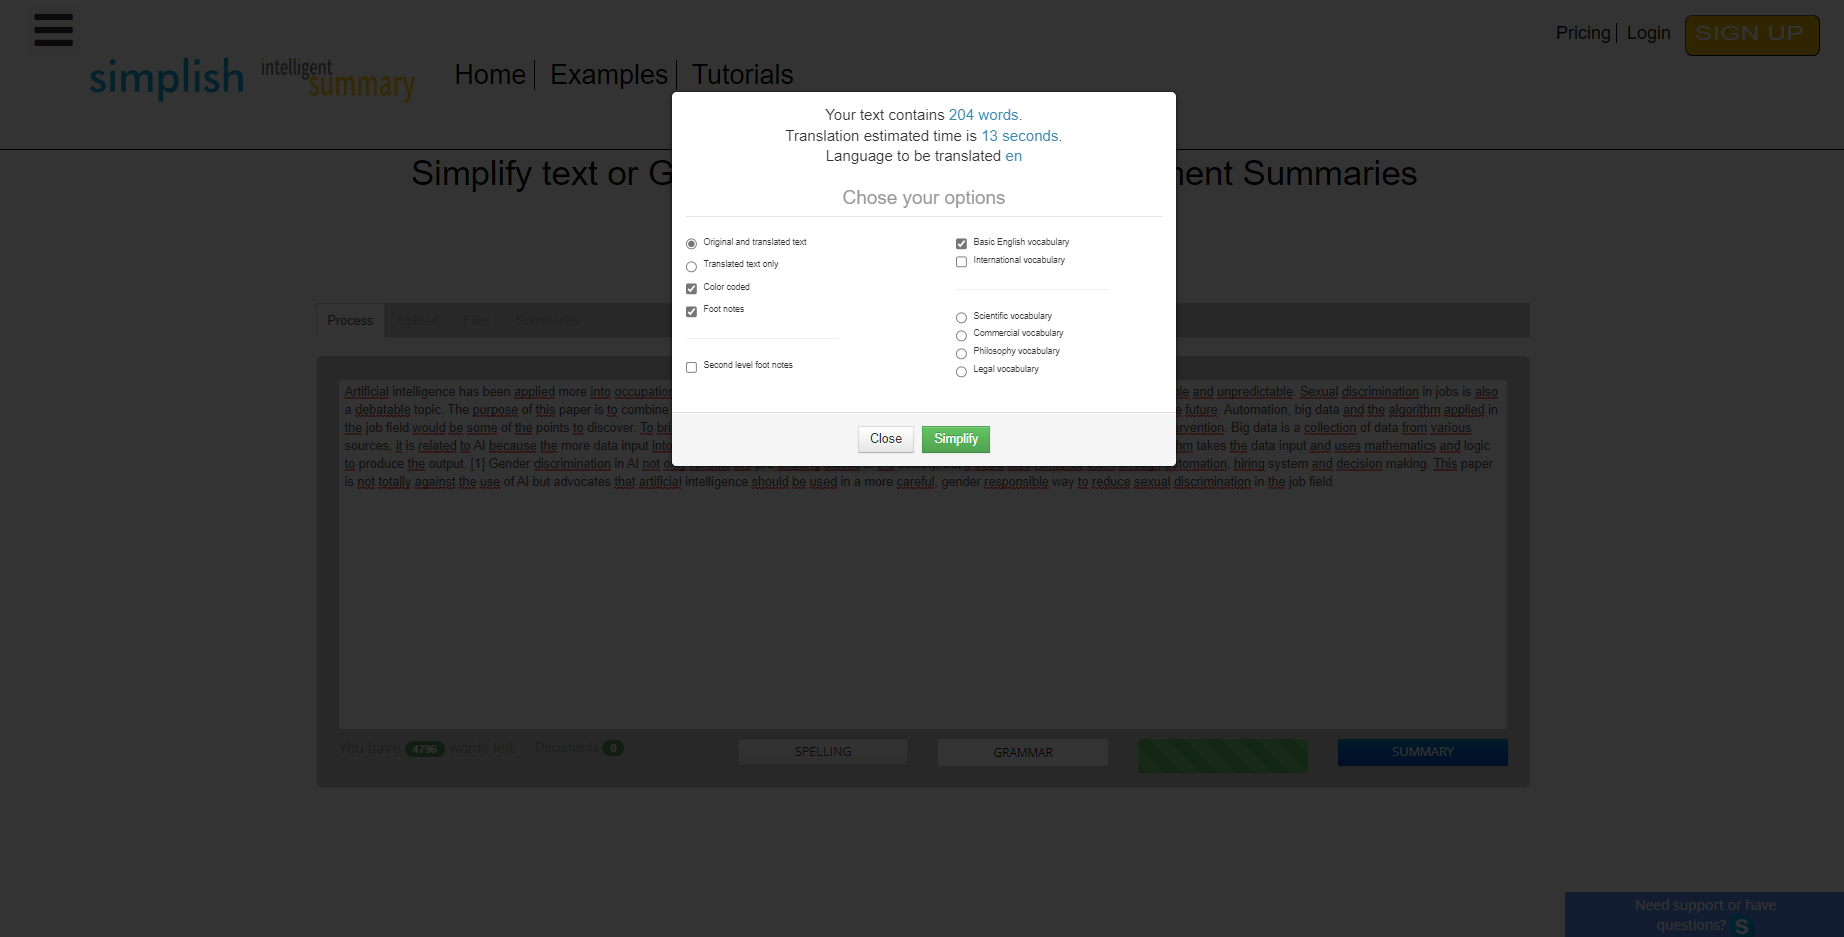
\includegraphics[width=\linewidth]{img/simplish-input.png}
\end{figure}

\begin{figure}[H]
	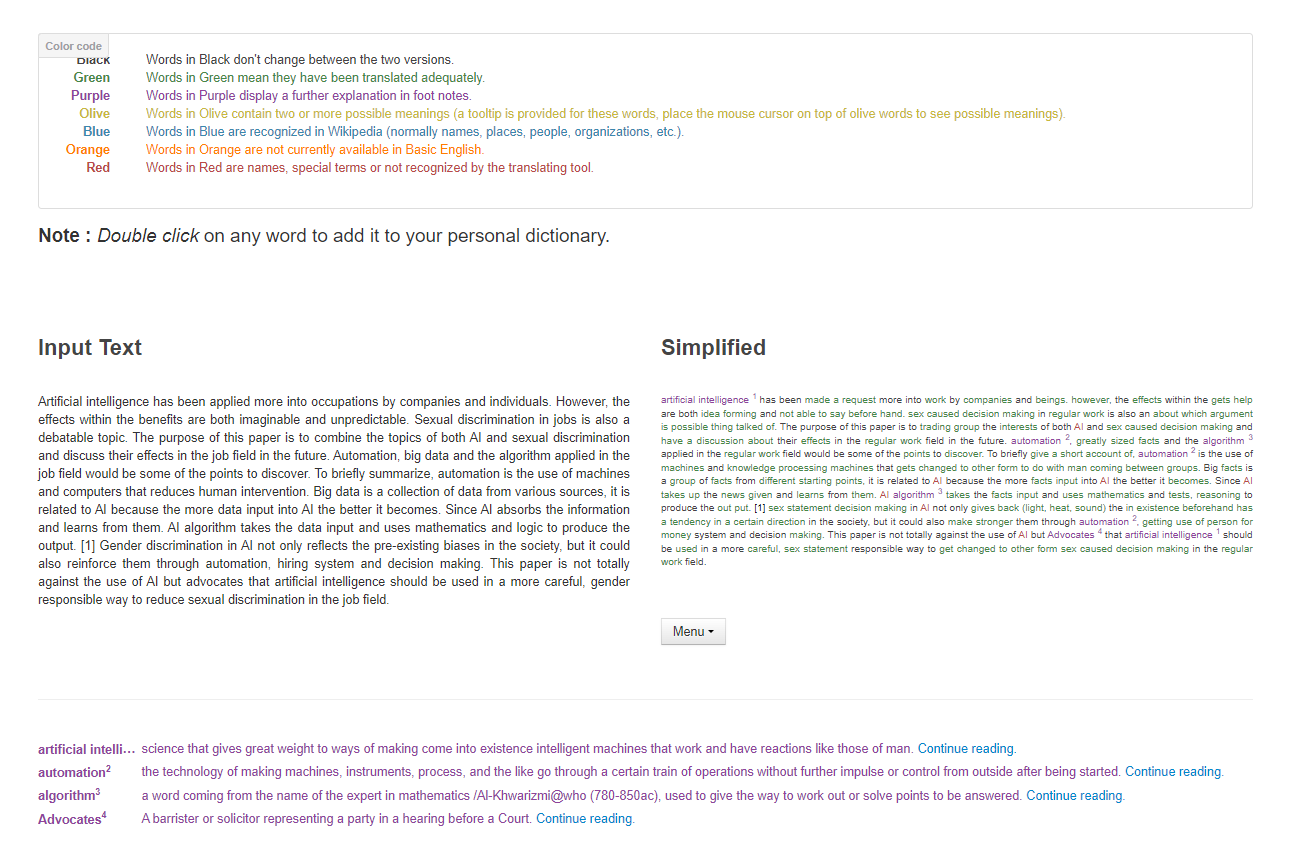
\includegraphics[width=\linewidth]{img/simplish-output.png}
\end{figure}

\section{Lexicale vereenvoudiging}

Huidige software in het onderwijs ingezet is in staat om woordenlijsten op te maken. Kurzweil biedt de functionaliteit om meer informatie te geven over een door de gebruiker gekozen woord, soortgelijk aan de werking van een woordenboek. Daarnaast biedt Kurzweil ook de mogelijkheid om als eindgebruiker de bron of woordenboek te kiezen waarvan de definitie moet worden opgehaald. Complexe woorden worden echter niet automatisch herkend door het systeem. Transformaties aan de woordenschat van een tekst komen in deze softwarepakketten niet aan bod.

\begin{table}[H]
	\centering
	\resizebox{0.8\textwidth}{!}{
	\begin{tabular}{|p{2cm}|l|l|l|l|l|l|}
		\hline
		Onderwerp & Mv & Sp & K3000 & AS & IW & TA \\ \hline
		Moeilijke woordenschat vervangen & X & - & - & - & - & - \\ \hline
		Glossary aanmaken (vak/wetenschappelijk jarg.) & X & X & X & X & - & - \\ \hline
		Synoniemenwoordenboek & X & - & X & - & - & - \\ \hline
		Verklarende (semantische) vereenvoudiging & X & - & - & - & - & - \\ \hline
		Identificeer complexe woorden & X & - & - & - & - & - \\ \hline
		Vervang complexe woorden door eenvoudigere synoniemen & X & - & - & - & - & - \\ \hline
		Gebruik een gecontroleerde en vertrouwde woordenschat; vermijd jargon & X & - & - & - & - & - \\ \hline
		Vermijd idiomatische uitdrukkingen & X & - & - & - & - & - \\ \hline
		Vermijd dubbelzinnige woorden & X & - & - & - & - & - \\ \hline
	\end{tabular}
}
\end{table}

Webapplicaties en -tools bieden meer functionaliteiten aan. Deze tools kunnen in rechtstreeks contact staan met online bronnen, zoals bij de Bing chatbot, of kunnen informatie ophalen vanuit riante datasets, zoals het GPT-3 model. De verwante GPT-modellen dienen expliciet aangewezen te worden om een tekst te kunnen vereenvoudigen. De redenering achter deze modellen is mogelijk om op te vragen, al vergt dit een bedachtzame prompt. Verwante GPT-modellen zijn in staat om rekening te houden met de dubbelzinnigheid van de woordenschat, alsook bij het rekening houden met wetenschappelijk of vakjargon. De prompt is bij deze modellen de doorslaggevende factor waarbij een bedachtzame voorbereiding moet worden toegediend door de gebruiker. Door deze vereisten te volgen, kan de tool de leesbaarheid van de tekst verbeteren en begrijpelijker maken voor een breder publiek.

\begin{table}[H]
	\centering
	\resizebox{0.8\textwidth}{!}{
	\begin{tabular}{|p{2cm}|l|l|l|l|l|l|l|l|l|}
		\hline
		Onderwerp & Mv & Ss & Sp & R & H & CGPT & GPT-3 & GPT-4 & B \\ \hline
		Glossary aanmaken (vak/wetenschappelijk jarg.) & X & - & X & - & - & + & + & + & + \\ \hline
		Synoniemenwoordenboek & X & + & X & - & - & + & + & + & + \\ \hline
		Verklarende (semantische) vereenvoudiging & X & + & X & - & X & + & + & + & + \\ \hline
		Complex Word Identification & X & X & X & - & X & X & X & X & X \\ \hline
		Complex Word Replacement & X & + & X & - & X & + & + & + & + \\ \hline
		Vervang complexe woorden door eenvoudigere synoniemen & X & + & X & - & X & + & + & + & + \\ \hline
		Gebruik een gecontroleerde en vertrouwde woordenschat; vermijd jargon & X & - & X & - & - & + & + & + & + \\ \hline
		Vermijd idiomatische uitdrukkingen & X & - & X & - & - & + & + & + & + \\ \hline
		Vermijd dubbelzinnige woorden & X & - & X & - & - & + & + & + & + \\ \hline
	\end{tabular}
	}
\end{table}


\section{Syntactische vereenvoudiging}

De huidige software transformeert de oorspronkelijke tekst niet. Daarmee is syntactische vereenvoudiging hier niet tot de orde.

\begin{table}[H]
	\centering
	\resizebox{0.8\textwidth}{!}{
	\begin{tabular}{|p{2cm}|l|l|l|l|l|}
		\hline
		Onderwerp & Mv & Sp & K3000 & AS & IW & TA \\ \hline
		Tangconstructies aanpassen & X & - & - & - & - & - \\ \hline
		Zinnen langer dan tien woorden inkorten. & X & - & - & - & - & - \\ \hline
		Verwijswoorden aanpassen & X & - & - & - & - & - \\ \hline
		Voorzetseluitdrukkingen vervangen & X & - & - & - & - & - \\ \hline
		Samengestelde werkwoorden vervangen & X & - & - & - & - & - \\ \hline
		Gebruik de actieve stem & X & - & - & - & - & - \\ \hline
		Vermijd onregelmatige werkwoorden & X & - & - & - & - & - \\ \hline
	\end{tabular}
}
\end{table}



\begin{table}[H]
	\centering
	\resizebox{0.8\textwidth}{!}{
	\begin{tabular}{|p{2cm}|l|l|l|l|l|l|l|l|}
		\hline
		Onderwerp & Mv & Ss & Sp & R & H & CGPT & GPT-3 & GPT-4 & B \\ \hline
		Tangconstructies aanpassen & X & - & - & - & + & + & + & + & + \\ \hline
		Zinnen langer dan tien woorden inkorten. & X & - & - & - & + & + & + & + & + \\ \hline
		Verwijswoorden aanpassen & X & - & - & - & + & + & + & + & + \\ \hline
		Voorzetseluitdrukkingen vervangen & X & - & - & - & + & + & + & + & + \\ \hline
		Samengestelde werkwoorden vervangen & X & - & - & - & + & + & + & + & + \\ \hline
		Gebruik de actieve stem & X & - & - & - & + & + & + & + & + \\ \hline
		Vermijd onregelmatige werkwoorden & X & - & - & - & + & + & + & + & + \\ \hline
	\end{tabular}
}
\end{table}

\section{Samenvatten}

De huidige tools in het onderwijs laten gebruikers toe om zinnen te markeren. Vervolgens worden deze gemarkeerde zinnen aan elkaar gekoppeld. De semantiek in de resulterende tekst blijft identiek, maar de resulterende tekst kan niet coherent zijn omwille van de extraherende samenvatting. Parafraseren of abstraherend samenvatten is echter niet mogelijk met software momenteel in het onderwijs beschikbaar. 

\begin{table}[H]
	\centering
	\resizebox{0.8\textwidth}{!}{
	\begin{tabular}{|p{2cm}|l|l|l|l|l|}
		\hline
		Onderwerp & Mv & Sp & K3000 & AS & IW & TA \\ \hline
		Bronvermelding & X & - & - & - & - & - \\ \hline
		Automatische markering van de belangrijke zinnen & X & - & - & - & - & - \\ \hline
		Automatische markering van de moeilijk leesbare zinnen & X & - & - & - & - & - \\ \hline
		Gemarkeerde zinnen samenvatten & X & X & X & X & X & X \\ \hline
		Gemarkeerde zinnen abstraherend samenvatten & X & - & - & - & - & - \\ \hline
		Automatische extraherende samenvatting & X & - & - & - & - & - \\ \hline
		Automatische abstraherende samenvatting & X & - & - & - & - & - \\ \hline
		Lengte van de samenvatting controleren door gebruiker & X & X & X & X & X & X \\ \hline
		Samenvatten op basis van kernwoorden & X & - & - & - & - & - \\ \hline
	\end{tabular}
}
\end{table}

Huidige tools maken gebruik van geavanceerde taalmodellen, zoals BERT of GPT-3. Dit leidt tot meer functionaliteiten waaronder abstraherend samenvatten op basis van gemarkeerde zinnen of woorden gekozen door de eindgebruiker. De experimenten met teksten wijzen uit dat GPT en Bing AI de nadruk legt op het behouden van bronreferenties. Wanneer expliciet gevraagd aan de Bing chatbot, geeft het model bronnen terug die buiten het oorspronkelijke artikel te vinden zijn. 

\begin{table}[H]
	\centering
	\resizebox{0.8\textwidth}{!}{
	\begin{tabular}{|p{2cm}|l|l|l|l|l|l|l|l|}
		\hline
		Onderwerp & Mv & Ss & Sp & R & H & CGPT & GPT-3 & GPT-4 & B \\ \hline
		Bronvermelding & X & - & - & - & - & + & + & + & X \\ \hline
		Automatische markering van de belangrijke zinnen & X & - & - & - & - & + & + & + & + \\ \hline
		Automatische markering van de moeilijk leesbare zinnen & X & - & - & - & - & + & + & + & + \\ \hline
		Gemarkeerde zinnen samenvatten & X & - & X & - & X & + & + & + & + \\ \hline
		Gemarkeerde zinnen abstraherend samenvatten & X & - & X & X & X & + & + & + & + \\ \hline
		Automatische extraherende samenvatting & X & - & X & - & X & + & + & + & + \\ \hline
		Automatische abstraherende samenvatting & X & X & X & - & X & X & X & X & X \\ \hline
		Lengte van de samenvatting controleren door gebruiker & X & X & X & - & + & + & + & + & + \\ \hline
		Samenvatten op basis van kernwoorden & X & - & - & - & - & + & + & + & + \\ \hline
	\end{tabular}
}
\end{table}

\section{Functionaliteiten}

\begin{table}[H]
	\centering
	\resizebox{0.8\textwidth}{!}{
	\begin{tabular}{|p{2cm}|l|l|l|l|l|}
			\hline
			Onderwerp & Mv & Sp & K3000 & AS & IW & TA \\ \hline
			Lettertype aanpassen & X & - & - & - & - & - \\ \hline
			Lettergrootte aanpassen & X & - & - & - & - & - \\ \hline
			Formaat aanpassen & X & - & - & - & - & - \\ \hline
			Achtergrondkleur aanpassen & X & - & - & - & - & - \\ \hline
			Browserextensie & nvt & - & - & - & - & X \\ \hline
			Exporteren naar PDF mogelijk & nvt & - & - & - & - & X \\ \hline
			Afbeeldingen uploaden & nvt & - & - & - & - & - \\ \hline
			Afbeeldingen lezen & nvt & X & X & X & X & X \\ \hline
			Afbeeldingen interpreteren & nvt & - & - & - & - & - \\ \hline
			Netwerkverbinding nodig & nvt & - & - & - & - & X \\ \hline
			Webapplicatie of online tool & nvt & X & - & - & X & X \\ \hline
			PDF/Word ondersteuning & nvt & X & X & X & X & X \\ \hline
	\end{tabular}}
\end{table}


\begin{table}[H]
	\centering
	\resizebox{0.8\textwidth}{!}{
		\begin{tabular}{|p{2cm}|l|l|l|l|l|l|l|l|}
			\hline
			Onderwerp & Mv & Ss & Sp & R & H & CGPT & GPT-3 & GPT-4 & B \\ \hline
			Lettertype aanpassen & X & - & - & - & - & - & - & - & - \\ \hline
			Lettergrootte aanpassen & X & - & - & - & - & - & - & - & - \\ \hline
			Formaat aanpassen & X & - & - & - & - & - & - & - & - \\ \hline
			Achtergrondkleur aanpassen & X & - & - & - & - & - & - & - & - \\ \hline
			Browserextensie & nvt & X & - & X & X & - & - & - & X \\ \hline
			Exporteren naar PDF mogelijk & nvt & - & - & X & - & - & - & - & - \\ \hline
			Afbeeldingen uploaden & nvt & - & - & - & - & - & - & X & X \\ \hline
			Afbeeldingen lezen & nvt & - & - & - & - & - & - & X & ~ \\ \hline
			Afbeeldingen interpreteren & nvt & - & - & - & - & - & - & X & ~ \\ \hline
			Netwerkverbinding nodig & nvt & X & X & X & X & X & X & X & ~ \\ \hline
			Webapplicatie of online tool & nvt & X & X & X & X & X & X & X & X \\ \hline
			PDF/Word ondersteuning & nvt & X & X & X & - & - & - & - & - \\ \hline
		\end{tabular}
	}
\end{table}

\section{Voor ontwikkelaars}

In mindere mate zijn er beperkingen voor de tekstsoftware die momenteel in het onderwijs wordt ingezet. Ontwikkelaars kunnen echter geen API aanspreken waarvan de volgende softwarepakketten gebruik maakt. Daarnaast is het niet mogelijk om te achterhalen van welk taalmodel de softwarepakketten gebruik maakt, of deze al dan niet aan bod komt.

\begin{table}[H]
	\centering
	\resizebox{0.8\textwidth}{!}{
	\begin{tabular}{|p{2cm}|l|l|l|l|l|}
			\hline
			Onderwerp & Mv & Sp & K3000 & AS & IW & TA \\ \hline
			Karakterlimiet & nvt & - & - & - & - & - \\ \hline
			Betalend & nvt & X & X & X & X & - \\ \hline
			API-sleutel nodig & nvt & - & - & - & - & - \\ \hline
			Betafase of wachtlijst & nvt & - & - & - & - & - \\ \hline
			Multilinguaal model & nvt & - & - & X & - & - \\ \hline
			White-box & nvt & - & - & - & - & - \\ \hline
			Black-box & nvt & - & - & - & - & X \\ \hline
		\end{tabular}
	}
\end{table}

Ontwikkelaars moeten rekening houden bij de karakter- of tokenlimiet bij alle modellen of tools. Dit hindert ontwikkelaars bij het ontwerpen en ontwikkelen van software waarbij grote documenten vanaf twee tot drie pagina's voltekst, moeten opgebroken worden in kleinere subdelen. Wetenschappelijke artikelen volgen een logische structuur, dus hier kunnen ontwikkelaars op inspelen. De meeste software is vrij beschikbaar, al zijn niet alle functionaliteiten vrij ter beschikking tot het grote publiek. De GPT-modellen, met uitzondering op chatbots, vereisen het gebruik van een API-sleutel. Het gebruik van deze sleutel is gekoppeld aan \textit{payment subscription} van OpenAI. Alle vermelde modellen maken gebruik van een black-box model. Geen taalmodel is ertoe in staat om duidelijk aan te geven waarom een zin als moeilijk wordt bestempeld, of waarom een woord als moeilijk werd bepaald. Dit sluit aan bij de bevindingen van \textcite{Gooding2022}. Black-box taalmodellen zijn dominant aanwezig, maar de zoektocht naar een white-box taalmodel van eenzelfde caliber is niet evident.

\begin{table}[H]
	\centering
	\resizebox{0.8\textwidth}{!}{
		\begin{tabular}{|l|l|l|l|l|l|l|l|l|}
			\hline
			Onderwerp & Mv & Ss & Sp & R & H & CGPT & GPT-3 & GPT-4 & B \\ \hline
			Karakterlimiet & nvt & 2048 & - & - & - & 2048* & 4096 & 4096 & 4096 \\ \hline
			Betalend & nvt & - & X & - & - & X & X & - & - \\ \hline
			API-sleutel nodig & nvt & - & - & - & - & X & X & X & X \\ \hline
			Betafase of wachtlijst & nvt & - & - & X & X & - & X & X & - \\ \hline
			Multilinguaal model & nvt & - & - & X & X & X & X & X & X \\ \hline
			White-box & nvt & - & X & - & - & - & - & - & - \\ \hline
			Black-box & nvt & X & X & X & X & + & + & + & + \\ \hline
		\end{tabular}
	}
\end{table}

\section{Conclusie}

Huidige tools hebben elk een eigen inbreng, maar er is geen manusje-van-alles. De toepassingen maken elk echter gebruik van beschikbare modellen en API's waarmee ontwikkelaars hiertoe in staat zijn. Op lexicaal en syntactisch vlak moet er een intuïtieve manier worden aangeboden voor gebruikers zodat zij niet aan prompt engineering hoeven te doen. Deze logica en bewerking kan in de vorm van een knop worden ingezet. 

Het prototype moet een duidelijke opsplitsing maken tussen de verwachtte functionaliteiten voor een scholier als voor een docent die een vereenvoudigde tekst maakt voor een scholier. Scholieren met dyslexie in de derde graad van het middelbaar onderwijs hebben nood aan een ondersteunende tool die hen toelaat om meer info rond zinnen of woorden op te halen, zodat zij de teksten beter kunnen lezen zonder dat de zinnen hun semantiek verliezen of zodat de scholieren niet de nodige kennis ontbreken zoals jargon of zinsstructuren. De docent daarentegen zal eerder een overzicht moeten kunnen krijgen van de oorspronkelijke tekst, alsook keuzes aangereikt moeten krijgen waaraan de vereenvoudigde tekst kan voldoen. De resulterende tekst is dan in de vorm van een PDF of online te bezichtigen.

\chapter{Prototype voor tekstvereenvoudiging}

\section{Voorbereiding}

\subsection{Python-notebooks}

De werking van tekstvereenvoudiging via Python-code wordt optimaal weergegeven in Python notebooks. Het gebruik van API's vormt geen hindernis en voorziet een snelle weergave zonder dat code uitgevoerd moet worden. 

\subsubsection{Keuze back-end en front-end}

Het prototype maakt gebruik van een Flask en het Jinja-framework. Aanvullend maakt het prototype gebruik van de nodige HTML- en CSS bestanden om de nodige visuele ondersteuning te kunnen aanbieden aan zowel lectoren als scholieren met dyslexie in de derde graad van het middelbaar onderwijs. Het aanspreken van de back-end vanuit de HTML-pagina's gebeurt met JavaScript-calls.

\subsubsection{Docker-omgeving}

Voor een optimale opzet als ontwikkelaar wordt er gebruik gemaakt van Docker. Een bat-scriptbestand maakt de opstart van deze lokale webapplicatie intuïtiever dan de opstart via een terminal. Daarnaast worden de benodigde Python-bibliotheken en taalmodellen alvorens opgehaald.

\subsubsection{PDF text mining}

De meest gebruikte vorm van tekstbestanden is in de vorm van PDF-bestanden. Methoden om deze bestanden uit te lezen en om te zetten naar tekstdata bestaan reeds in de vorm van Python-bibliotheken. De keuze van de bibliotheek speelt wel een rol. Sommige Python-bibliotheken bieden meer analyse- en verwerkingsfuncties aan. PDF Miner biedt extra functies aan om de metadata van een PDF-bestand op te halen of om classificatie op basis van lettertypes of pagina's per titel op te halen. Deze functies bevatten een intuïtieve naamgeving en besparen ontwikkelaars de overbodige werklast om extra logica te schrijven.

\subsubsection{Data pre-processing}

% todo stopword removal voor keyword extraction

\subsection{Extraherende samenvatting}

\subsubsection{BERT Extractive Summarization}

Indien niet aangegeven, wordt het aantal zinnen bepaald door het BERT-model.

\subsubsection{Vertaling}

BERT houdt geen rekening met vertaling. Het model staat enkel paraat om zinnen te markeren en de belangrijkste zinnen terug te geven. Voor de vertaling wordt de Google Translate Python-package gebruikt. Deze is minder accuraat vergeleken met DeepL, maar biedt een gratis beschikbaar en aanvaardbaar alternatief aan. Factoren zoals topic diversity en semantische redundantie moeten overwogen worden bij het kiezen van een taalmodel voor extraherend samenvatten.

\begin{lstlisting}[language=Python]
def extractive_summarization(full_text):

try:    
    from summarizer import Summarizer
    model = Summarizer()

    """determining optimal number of sentences based on MMR"""
    res = model.calculate_optimal_k(
        full_text, 
        k_max=10
    )

    """extracting key sentences"""
    result = model(
        body=full_text,
        max_length=700,
        min_length=100,
        num_sentences=res,
        return_as_list=True
    )

    new = []
    try:
        for i in result:
            if detect(i) != LANG:
                new.append(translate_sentence(i))
            else:
                new.append(i)
        return ' '.join(new)
    except Exception as e:
        return f'Problemen met Google Translate {e}'

except Exception as e:
    return f'Problemen met BERT {e}'
\end{lstlisting}

\subsection{Integreren naar Flask}

Flask biedt een snelle en toegankelijke opzet aan voor Python-ontwikkelaars. De combinatie van een robuuste front-end en back-end maakt dit binnen de schaal van een prototype ideaal.

\begin{lstlisting}

@app.route('/', methods=['GET'])
def home():
	return render_template('index.html')

if __name__ == "__main__":
	app.run()
\end{lstlisting}

% \subsection{title}

